%!TEX root = informe.tex
En este contexto, consideraremos \emph{artifacts} a aquellos errores visuales resultantes de la aplicaci\'on de un m\'etodo o t\'ecnica. En particular a aquellos que no reflejan una situación verosímil en la vida real\footnote{Esto es muy subjetivo, y no nos explayaremos más porque bordea la filosofía. Esperemos quede claro con los ejemplos.}.

Dividiremos nuestro análisis en diferentes casos, en función de las siguientes variables:
\begin{itemize}
	\item Método utilizado para la interpolación
	\item Tipo de movimiento grabado por la cámara
	\item Tipo de movimiento de la cámara
	\item En el caso de splines, tamaño del bloque utilizado
\end{itemize}

Los algoritmos utilizados para producir el efecto de cámara lenta pueden clasificarse en los siguientes tipos:
\begin{itemize}
	\item Métodos predictivos: Interpolación polinomial de frames intermedios, intenta \emph{llenar los huecos} de forma natural entre cada par de frames, intentando predecir el comportamiento del video entre 2 frames conocidos.
	\item Métodos no predictivos: Vecino más cercano, se limita a copiar frames, sin interés en generar nueva información.
\end{itemize}

\emph{Nota:} Se consideran los videos del directorio subido a Google Drive adjunto con esta entrega. Para los 3 metodos de interpolacion se experimentó con los mismos videos.

\subsubsection{\bf{Interpolación por vecino mas cercano}}
Dado que este método de \emph{slowmotion} es un método \emph{no predictivo} no se producirán artifacts bajo nuestra definición, simplemente el video ralentizado tendrá un efecto de \texttt{lag} en donde la reproducción parece trabada. Esto es esperable, ya que este método copia frames consecutivamente para lograr un efecto de mayor tiempo de visualización por frame en la reproducción en tiempo real. 

\subsubsection{\bf{Interpolación lineal}}
\subsubsection*{Cámara fija e imagen fija - Caso de laboratorio}
En nuestro caso de laboratorio\footnote{Un video conteniendo un único frame repetido muchas veces.} puede observarse que al ser todos los pares de frames iguales los frames interpolados linealmente también lo serán ya que la recta que une a todos los píxeles entre los 2 frames consecutivos es una constante. No se observan artifacts.

\subsubsection*{Cámara fija e imagen fija}
Consideremos en este caso, un video de un objeto inmóvil, pero con cambios de iluminación. Lo que observamos es que a medida que vamos aumentando el factor de ralentización\footnote{Agregando mas frames intermedios.} se van suavizando los cambios en el video. Puntualmente, en el video original, observamos el suave cambio de color del cielo y el rápido encendido y apagado de luces. En el video ralentizado, mientras más frames fueron agregados artificialmente, se produce un efecto de suavizamiento de estos cambios rápidos, dándoles una sensación de transición lenta entre encendido y apagado de luces. Respecto a los cambios lentos, no observamos nada muy evidente.

\subsubsection*{Cámara fija e imagen móvil}
En este caso, se considera una cámara en posición fija, captando una escena con mucho movimiento y fondo estático. Particularmente es una escena de un partido de fútbol. Puede observarse que al aumentar el factor de \emph{slowmotion} se observa un efecto de \texttt{fantasmeo} en la parte móvil de la escena. Esto puede explicarse desde un punto de vista de la clasificación en métodos predictivos. Bajo el objetivo de construir una secuencia verosímil de frames entre dos frames consecutivos\footnote{En nuestro caso simplemente los \texttt{motion vectors} mapean idénticamente los píxeles entre dos frames consecutivos\cite{motion}.}, intenta predecir el movimiento de los objetos presentes, mientras menos distancia se mueva el objeto entre par de frames originales, mas acertada será esta predicción. Por otro lado, al estar mapeando los píxeles idénticamente al predecir el movimiento, nos queda esta sensación de fantasmeo, producida por la transición suave entre los colores en la región donde se produce el movimiento. Otro buen ejemplo donde se ve esta anomalía es la figura \ref{fig:lineal}, corrida sobre el video \emph{city.avi}. Respecto al fondo estático, al ser los valores de los píxeles iguales entre frames, la recta que los une también es constante y dichos píxeles son copiados idénticamente en cada frame agregado.

\begin{figure}[H]
    \centering
    \subfloat[][]{
        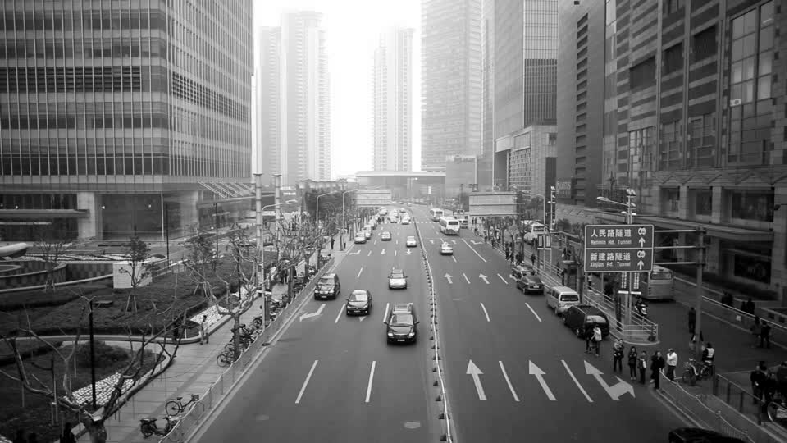
\includegraphics[width=.3\textwidth]{artiframes/camarafija_imagenmovil/frame001.pdf}
    }
    \subfloat[][]{
        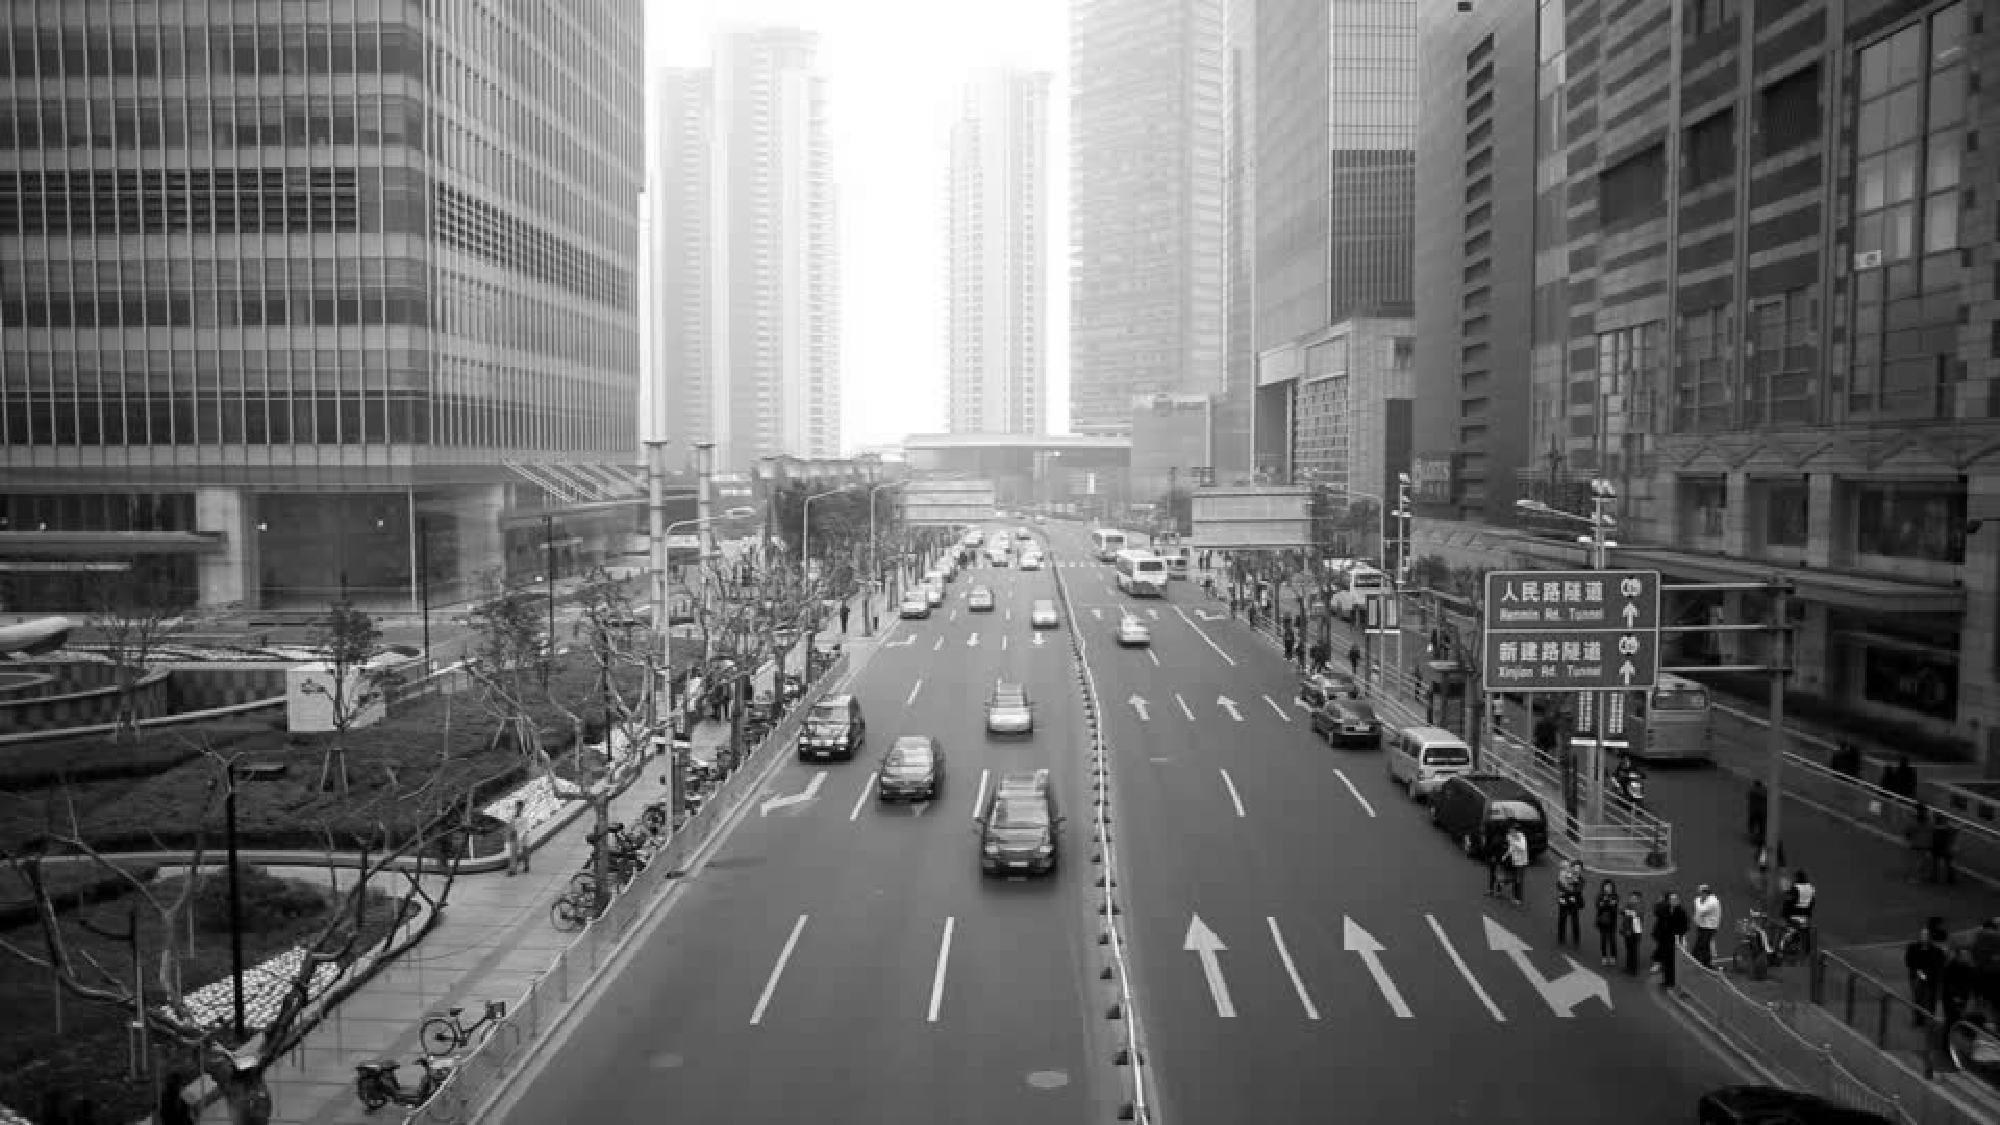
\includegraphics[width=.3\textwidth]{artiframes/camarafija_imagenmovil/frame003.pdf}        
    }
    \subfloat[][]{
        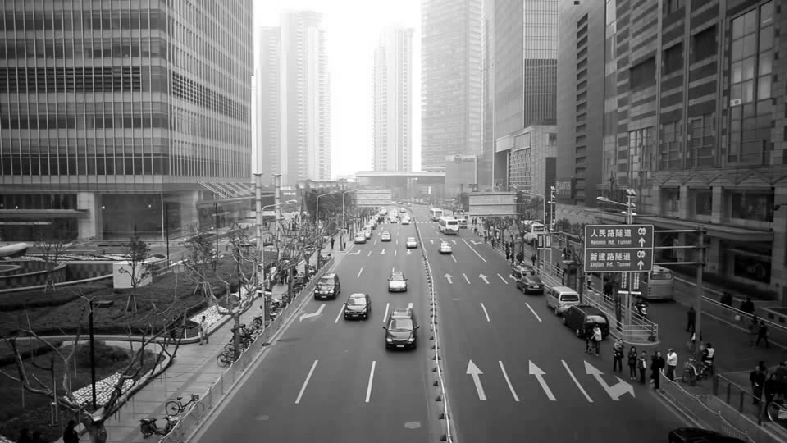
\includegraphics[width=.3\textwidth]{artiframes/camarafija_imagenmovil/frame007.pdf}        
    }
    \caption{Efecto de fantasmeo en interpolacion lineal}
    \label{fig:artifact}
\end{figure}


\begin{figure}[H]
    \centering
    \subfloat[][]{
        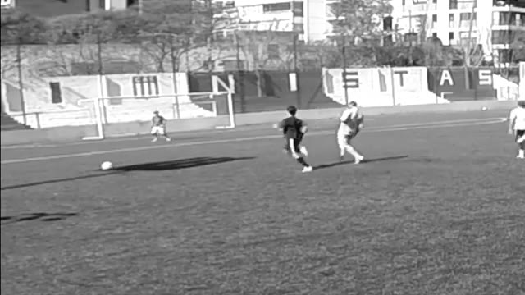
\includegraphics[width=.3\textwidth]{artiframes/camarafija_imagenmovil/frame445.pdf}
    }
    \subfloat[][]{
        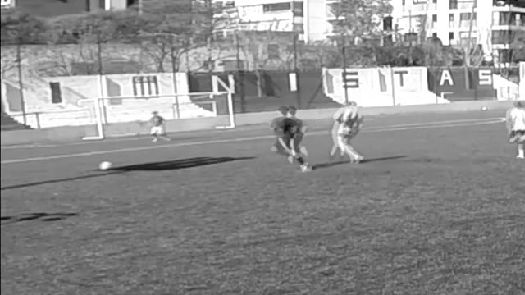
\includegraphics[width=.3\textwidth]{artiframes/camarafija_imagenmovil/frame448.pdf}        
    }
    \subfloat[][]{
        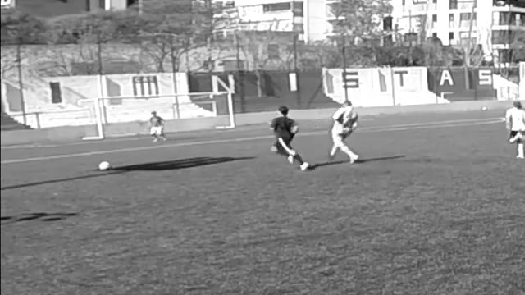
\includegraphics[width=.3\textwidth]{artiframes/camarafija_imagenmovil/frame451.pdf}        
    }
    \caption{Efecto de fantasmeo en interpolacion lineal}
    \label{fig:artifact}
\end{figure}


\begin{figure}[H]
    \centering
    \subfloat[][]{
        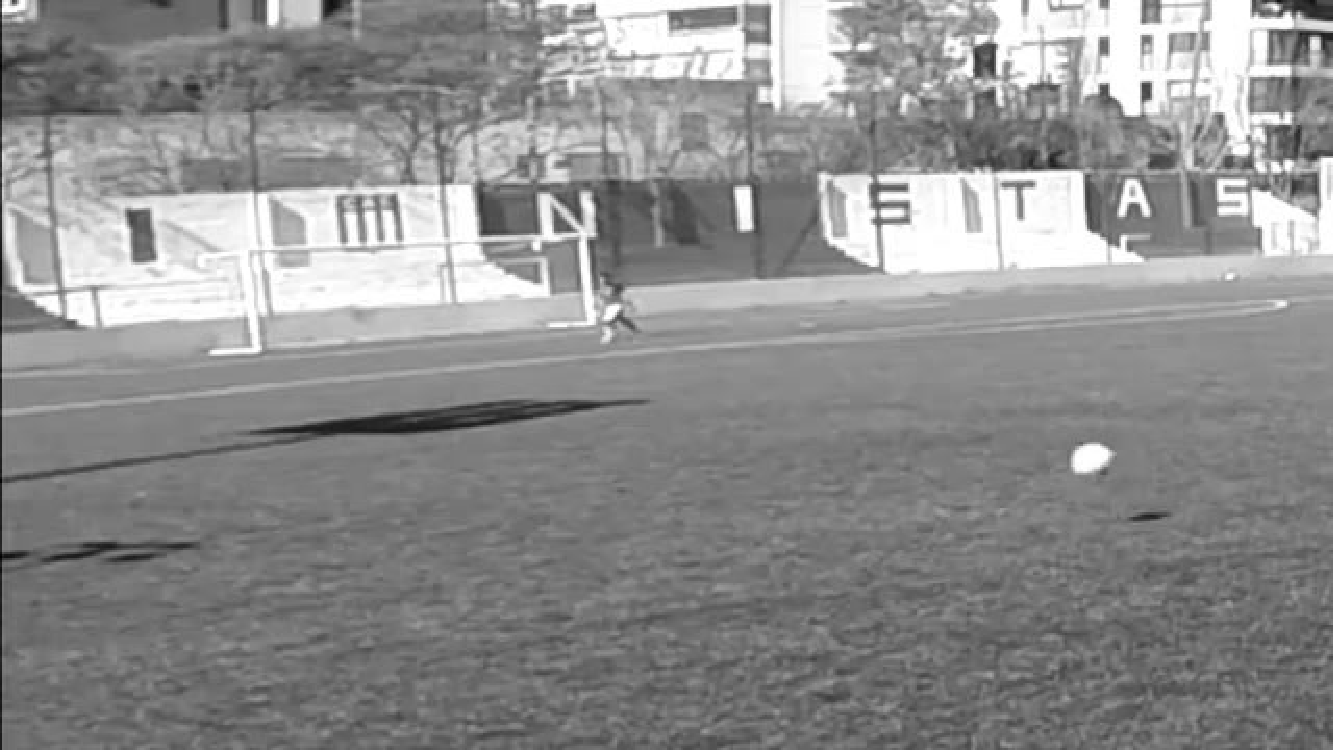
\includegraphics[width=.3\textwidth]{artiframes/camarafija_imagenmovil/frame145.pdf}
    }
    \subfloat[][]{
        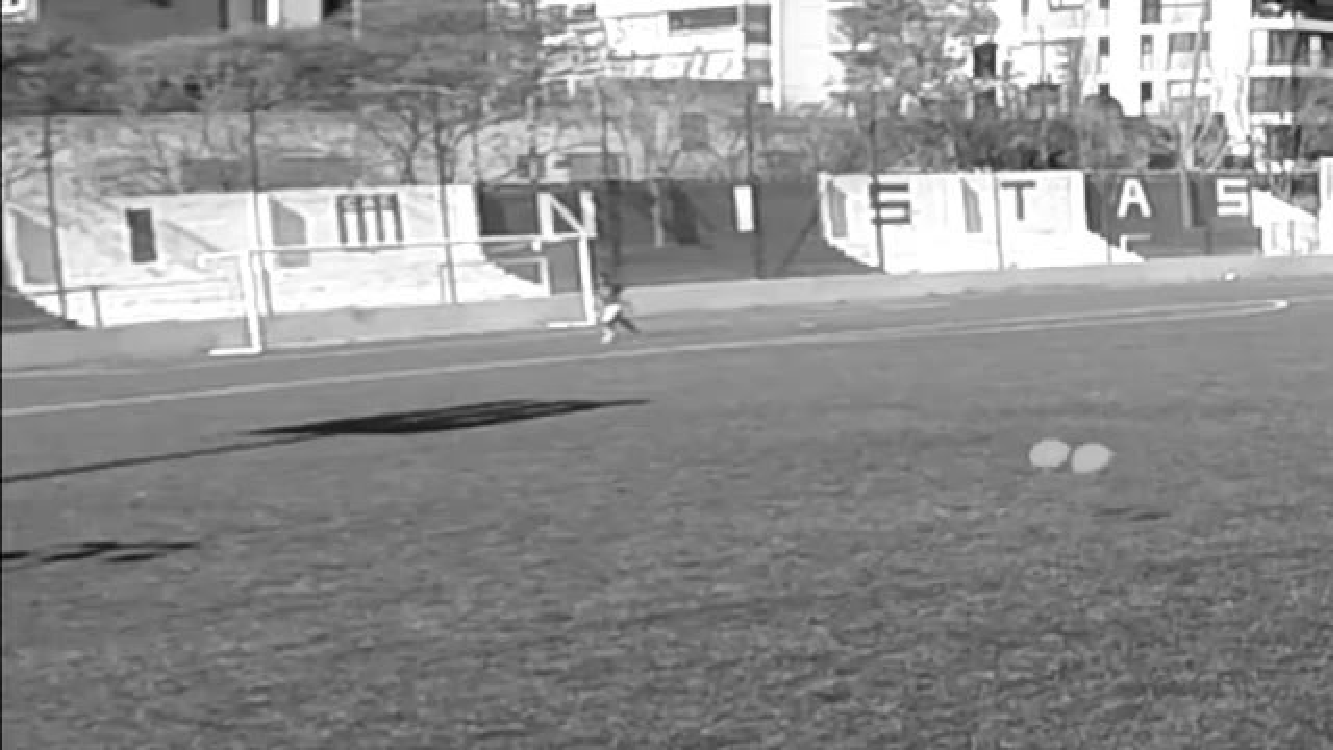
\includegraphics[width=.3\textwidth]{artiframes/camarafija_imagenmovil/frame148.pdf}        
    }
    \subfloat[][]{
        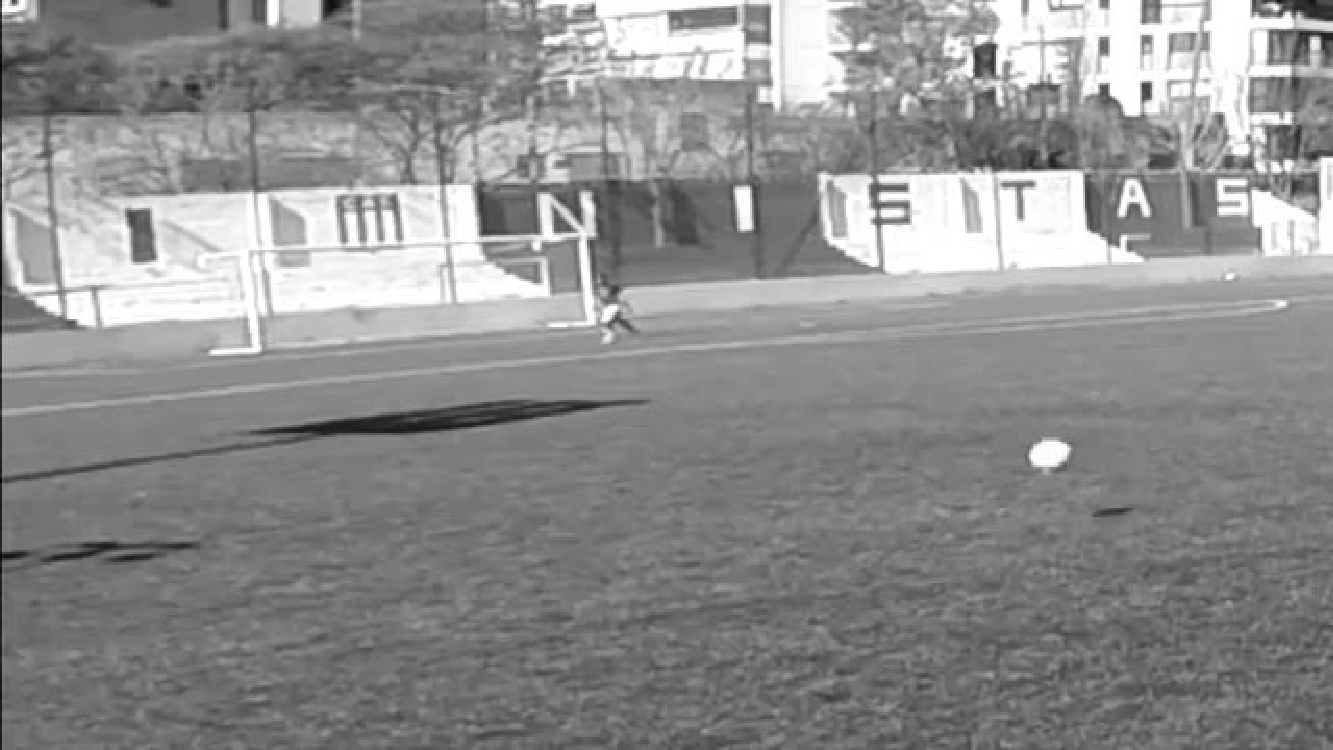
\includegraphics[width=.3\textwidth]{artiframes/camarafija_imagenmovil/frame151.pdf}        
    }
    \caption{Efecto de fantasmeo en interpolacion lineal}
    \label{fig:artifact}
\end{figure}

\subsubsection*{Cámara móvil e imagen fija}
En este caso lo que se observa es algo similar a lo mencionado anteriormente de \emph{motion prediction}, al moverse la figura, particularmente en los bordes de la misma, donde la diferencia entre el gris de la figura y el fondo negro es mas visible, se producen artifacts de fantasmeo mas marcado, nuevamente esto es producido por nuestro mapeo idéntico de píxeles entre frames, produciendo una transición suave de colores en las regiones donde se producen los cambios mas bruscos. El fondo no presenta artifacts evidentes. Como detalle, notar que en la parte frontal central del robot, los artifacts son mas leves, asumimos que esto se debe a que a pesar de mapear idénticamente los píxeles, la varianza de color de la región es muy baja.

\subsubsection*{Cámara móvil e imagen móvil}
Este caso de prueba se caracteriza por rápidos cambios en los ángulos de la filmación y por una escena rápida ocurriendo de fondo. Probablemente este sea el peor caso, cualitativamente hablando. Lo que se observa es que a medida que se aumenta el factor de ralentización, el video reconstruido sufre mucho más el hecho de predecir el movimiento con un mapeo idéntico de píxeles entre frames. Casi que para valores altos de ralentización es casi imposible de seguir el movimiento correcto ya que aparecen cosas que al ojo humano le parecerían dobles figuras\footnote{Por ejemplo cuando la pelota y la cámara se mueven al mismo tiempo, parece que hay varias pelotas.}

\begin{figure}[H]
    \centering
    \subfloat[][]{
        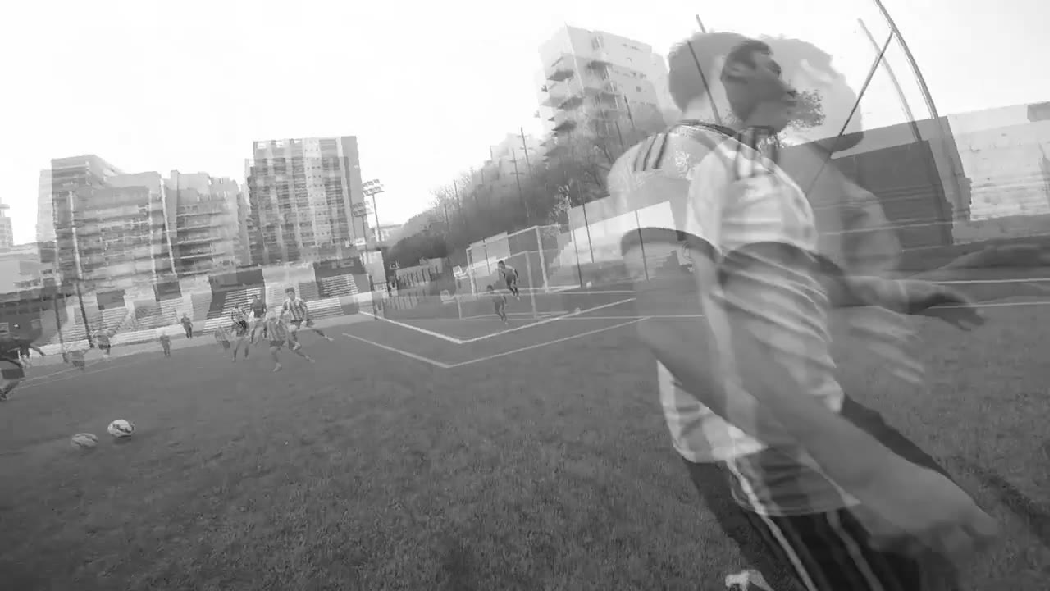
\includegraphics[width=.5\textwidth]{artiframes/movil_movil/frame113.pdf}        
    }
    \subfloat[][]{
        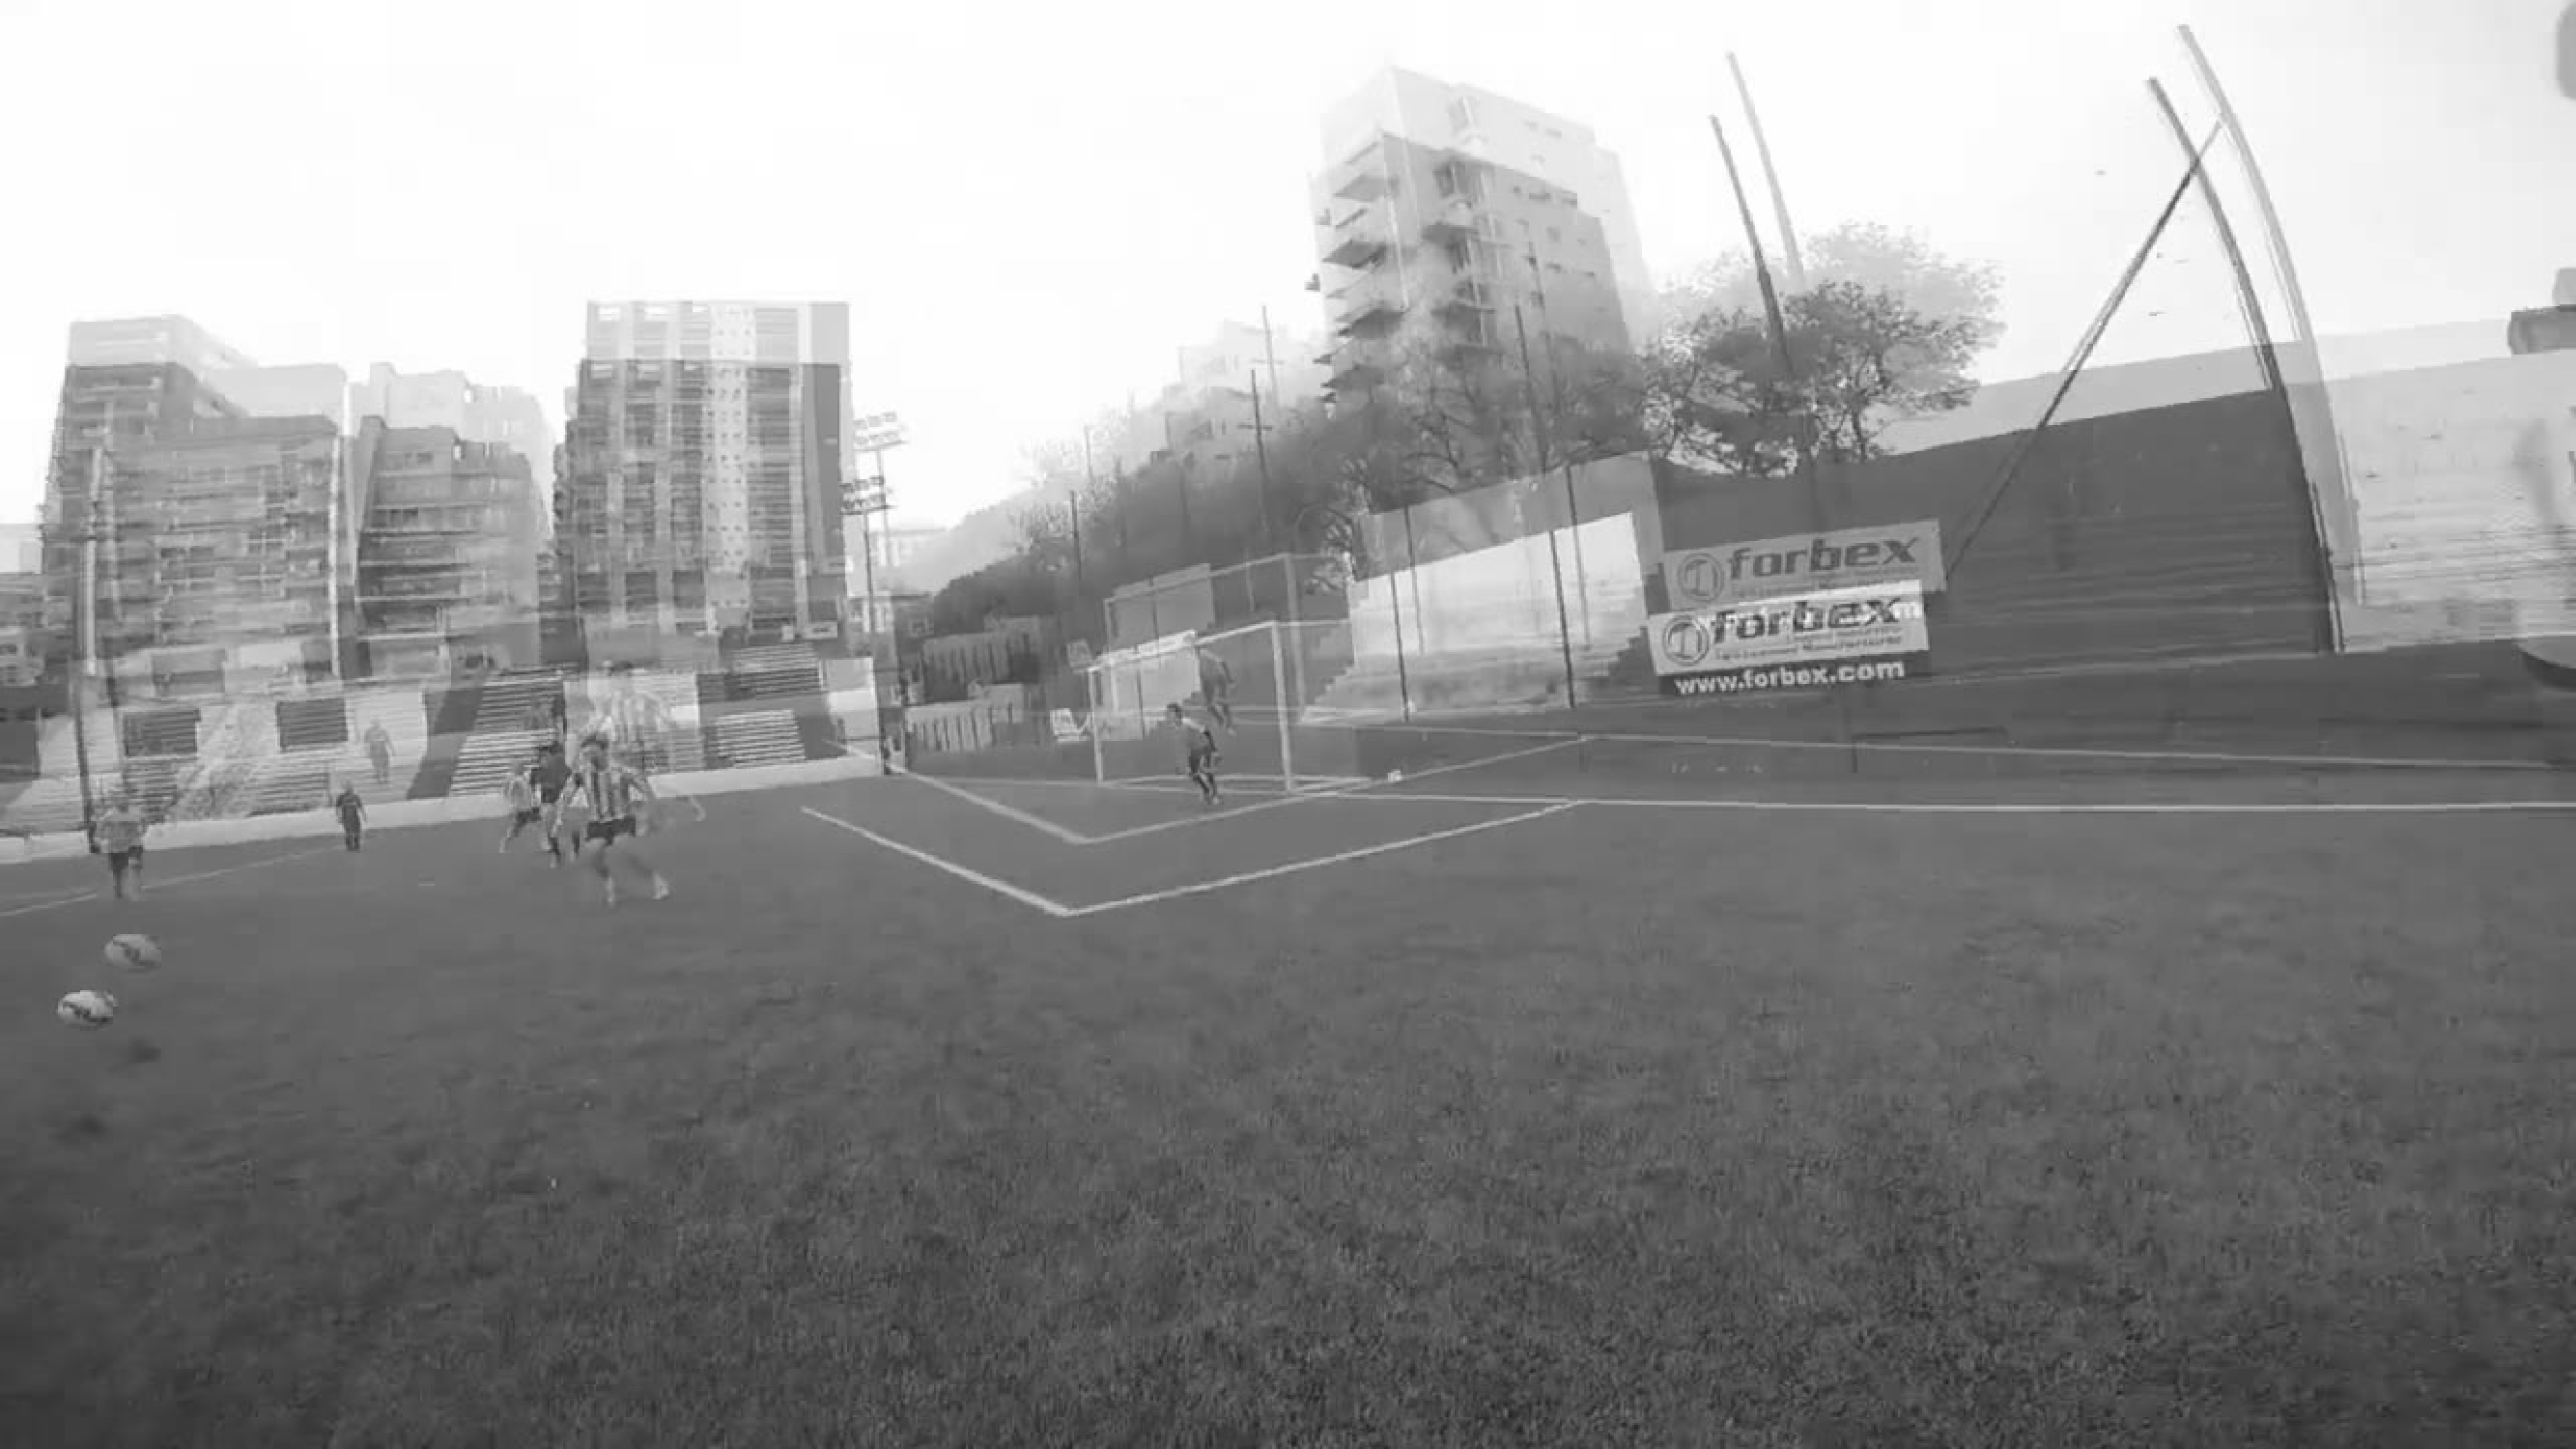
\includegraphics[width=.5\textwidth]{artiframes/movil_movil/frame117.pdf}
    }
    \caption{Dobles figuras en interpolacion lineal}
    \label{fig:artifact}
\end{figure}

\subsubsection*{Transición rápida de blanco a negro}
Mas allá del fantasmeo producido por la predicción del movimiento errónea, los cambios rápidos de blanco a negro, agregan un, si se quiere, natural degradé entre blanco y negro pasando por gris. Sin embargo, en la realidad, esto no necesariamente ocurre. Este método agrega un efecto espurio a al reacción química mostrada en el video.

% --------------- Splines ------------------

\subsubsection{\bf{Interpolación cúbica con splines}}
\subsubsection*{Cámara fija e imagen fija - Caso de laboratorio}
Sea $splBlk$ el tamaño del bloque de spline utilizado. Nuevamente en este caso puede observarse que al ser todos los pares de frames iguales los frames interpolados cubicamente también lo serán ya que el polinomio que une a todos los píxeles entre los $splBlk$ frames consecutivos es una constante. Dado que los bloques comparten el primer y ultimo frame, durante todo el video tambien se mantendra constante el valor de los píxeles. No se observan artifacts.

\subsubsection*{Cámara fija e imagen fija}
Los efectos en términos de artifacts de ralentizacion observados para los tamaños de bloque spline $splBlk = 8, 16$ son similares a los propuestos para interpolación lineal, los fondos estáticos no presentan artifacts, las transiciones rápidas como el encendido y apagado de luces fueron suavizadas y las transiciones lentas como el paso del dia son sutilmente mas suaves ya que como vimos en la sección de desarrollo la interpolacion por splines evita los picos en la interpolación fragmentada, otorgando una curva suave.

\subsubsection*{Cámara fija e imagen móvil}
En este caso, se considera nuevamente la escena de un partido de fútbol. Puede observarse que al aumentar el factor de slowmotion, los fondos estáticos quedan sin artifacts pues sus píxeles son copiados exactamente entre frames. Lo distinto respecto a interpolación lineal es que en lugar de un \emph{fantasmeo} lo que vemos es como una \emph{proyeccion al futuro y al pasado} del movimiento rápido de los objetos como la pelota. En particular las personas corriendo tienen un halo alrededor\footnote{\url{https://www.youtube.com/watch?v=Qw7F2MVFi1I}}. Esto se ve amplificado proporcionalmente a la ventana de spline que utilicemos y a la cantidad de frames a interpolar entre pares existentes de frames. Creemos que las caracteristicas de interpolacion por splines hacen un mejor intento por aproximar cosas intermedias usando mas información pero dado el mapeo idéntico de píxeles entre frames utilizado para predecir las trayectorias de los objetos en movimiento se produce este efecto de \emph{halo}. Al final del video puede verse que si las personas van caminando, el efecto de cámara lenta es mucho mejor y casi no tiene artifacts.
Si se revisa el experimento realizado sobre el video \emph{city.avi} se encontrara el efecto de halo muy visible en los autos que van a alta velocidad. 

\begin{figure}[H]
    \centering
    \subfloat[][]{
        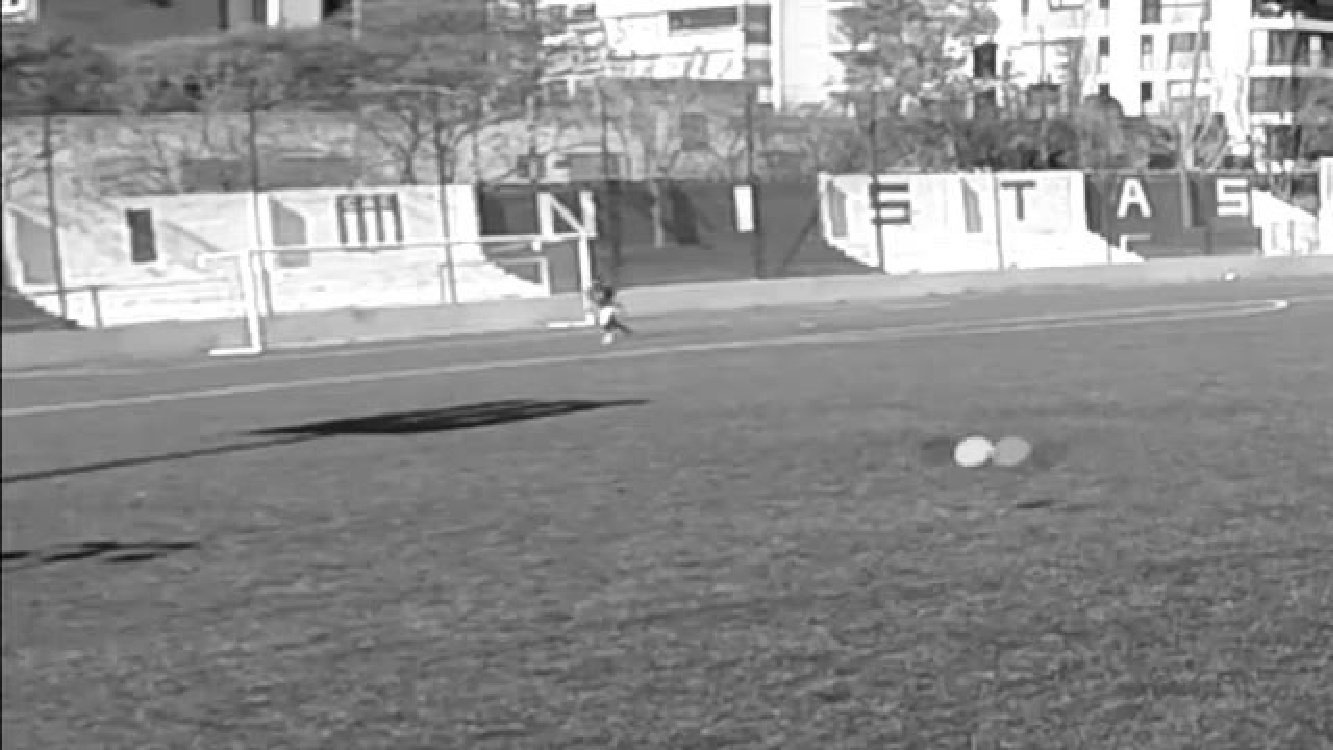
\includegraphics[width=.3\textwidth]{artiframes/splines_fija_movil/frame009.pdf}        
    }
    \subfloat[][]{
        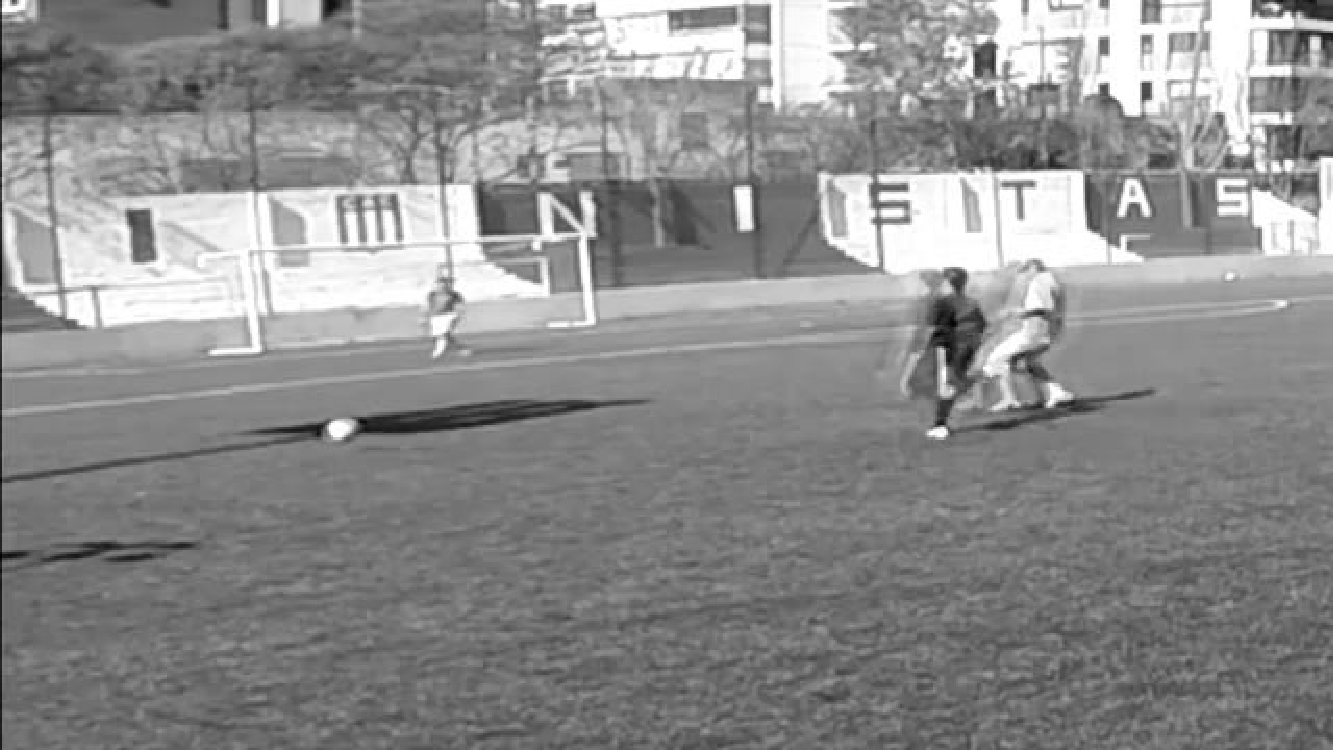
\includegraphics[width=.3\textwidth]{artiframes/splines_fija_movil/frame017.pdf}
    }
    \subfloat[][]{
        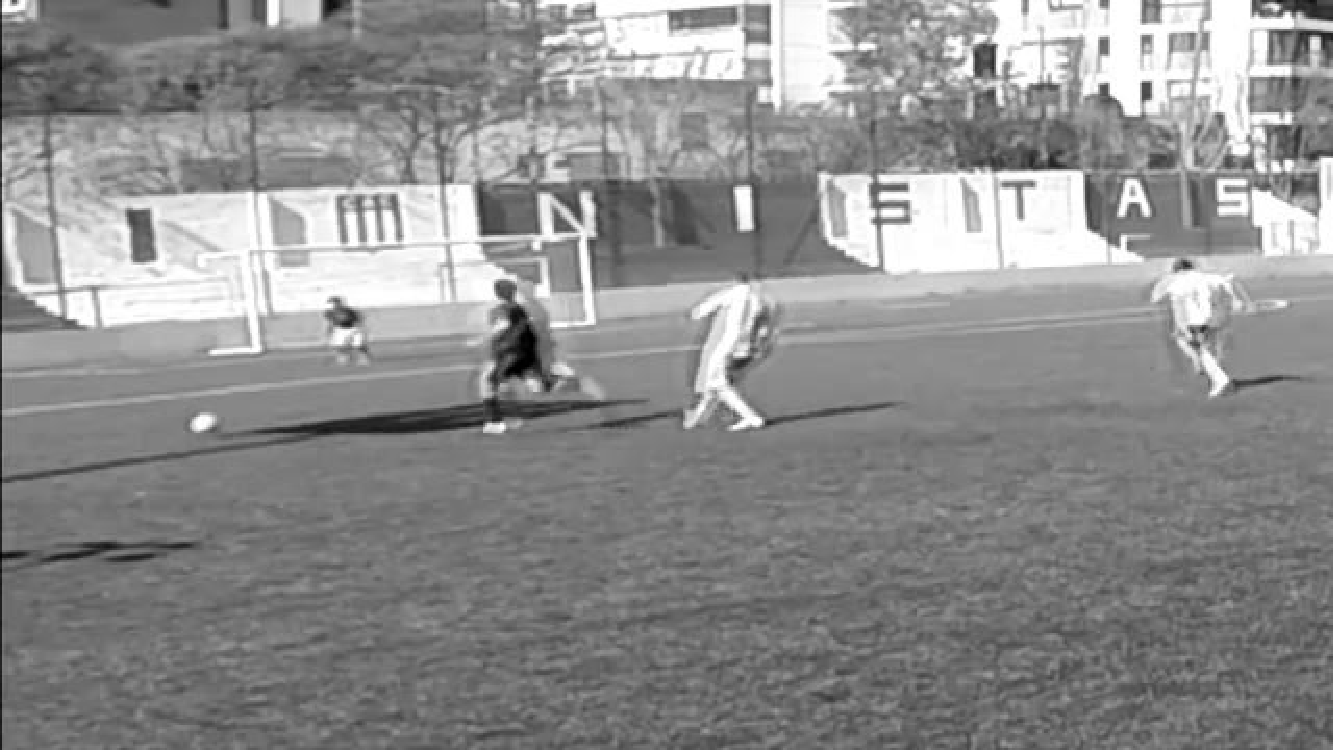
\includegraphics[width=.3\textwidth]{artiframes/splines_fija_movil/frame021.pdf}
    }
    \caption{Efecto halo figuras en interpolacion cúbica}
    \label{fig:artifact}
\end{figure}

\subsubsection*{Cámara móvil e imagen fija}
Este caso presenta artifacts muy similares a la interpolación lineal. Tal vez para una cantidad pequeña de frames a interpolar splines se comporta sutilmente mas suave.

\subsubsection*{Cámara móvil e imagen móvil}
Aqui nuevamente se presenta el peor caso en términos cualitativos, los cambios rápidos en el ángulo de filmación y simultáneo rápido movimiento de los objetos provocan un efecto extremo de \emph{halo}. Haciendo el video casi inservible si se quisiera analizar la cámara lenta. Se puede observar el halo por ejemplo en las líneas del arco, que tienen artifacts indicando una especie de sombra negra. 

\subsubsection*{Transición rápida de blanco a negro}
Este video es el mejor logrado de los analizados, su movimiento suave y fondo estático lo hacen perfecto para este tipo de \emph{motion prediction}. Para todas las combinaciones de $splBlk$ y $j$ cantidad de frames a interpolar entre pares, el video ralentizado parece muy natural. Sin embargo, como dijimos antes, aunque parezca natural, no necesariamente es lo que ocurre en la vida real.

